\documentclass{ltjsbook}
\usepackage{docmute} 
\usepackage{../../myStyle} 

\begin{document}
\setcounter{chapter}{2}
\chapter{社会心理学の歴史2;人文科学の知}
\label{sp03_humanities}
\section{振り返り}
それでは，時間になりましたのでお話を始めようと思います。まず，LMSの方で，いろいろご意見ご感想等をいただきましたので，それにお返事しようかなと思っています。
前回は，私も喋ってみて思ったんですけど，普段僕が90分授業をやっているものですから，こちらの105分授業がまだちょっと身体に馴染んでいなくて，最後の15分くらいか，そのちょっと前くらいから，頭が惚けてしまっていたというか，うまく話せていなかったような気がします。すみません。何の話かよくわからないような話を聞かせていしまって，皆さんも困ったかと思うんですが，そのようなご指摘もいただきまして。すみません。

さて，「量子力学の話とか知っていたけれども，科学における客観性とつなげて考えたことがなかった」とかですね，「心理学の考え方というのが，この量子力学の考え方に似ているのかな」とか，「いろいろ考えることができてよかった」というコメントをいただきました。ありがとうございます。

また，前回はいちおう社会心理学\index[termidx]{しゃかいしんりがく@社会心理学}の歴史の授業だったので，「心理学とかその前の科学とは何か」という話と，「どうつながっているのかが分かりにくかった」というようなご意見をいただきました。ごもっともだと思います。今日はちょっと，もうちょっとましな話ができればいいかなと思っています。
「社会心理学\index[termidx]{しゃかいしんりがく@社会心理学}の具体的な実験についていろいろ聞いたことがあって，もう少し深掘りしていただければ」というようなご意見もいただきました。もちろんそれもいいかなと思うんですけれども，講義録の方に引用文献を載せておきました。心理学の実験については，僕は授業中にも紹介したかもしれませんが，「心は実験できるか」という本\parencite{jikken2004}が面白かったのでご参照ください。テキスト教科書的な内容でよければ，そういったところを見ていただければと思います。もう少し詳細に書いているかと思いますので。皆さんは是非，この授業で聞いたことは，鵜呑みにせずいてほしいというか，ここで聞いたところの話で止まるのではなくて，そこからぜひ色々ご自身で深掘りしていっていただければと思います。

さて，もう一つ，講義を聞いていて，「なぜサイエンスになることが重要なのか」「なぜ客観性が重要なのか」ということについて深く考えていないからよくないのではないか，というご意見をいただきました。続けて，「教義として客観性が大事」という程度で止まっているのではないか，というようなご意見もいただきました。これを書いてくれた人は続けて，「個人的には予測や操作を可能にするためにそれが必要なんだ」というように書いておられます。「予測と制御」は確かに科学の一大目的の一つでして，それが少なくとも物理学が成功した一番の理由だとは思います。ただそれだけではなくて，今日の話の内容とも関係するのですが，科学というものを考えるときに，「人文社会科学的な知識」「知恵のある知のあり方」というのを考えてみたいと思うわけです。そうすると必ずしも「予測と制御」ということが目的ではないのではないかと思います。

この辺は「予測や制御しないサイエンス」というのはおかしい，という意見もあり得ると思いますし，一方で「知識」「知恵のある知のあり方」として「予測と制御しかない」というのも極端で，それだけではないのではないかとも，僕なんかは思います。もう一つ，「合理的な説明」ですとか，「あるいはより多くの人が納得できる説明の方法を与える」というのも，おそらくサイエンスの仕事の一部だと考えています。もちろん，今の言い方にはちょっと語弊，というか危険性もはらんでいるかな，というのはうすうす気づきながら話しているのですが，そのようなところ，客観性の持ち方と生活の知，生きているということの上での知識のあり方というのが，予測と制御だけでよいのか，というようなことについても考えていけるようになればなと思っています。

あと，この授業の見通しがちょっとつきにくいというお話もありまして，非常に恥ずかしい気持ちでいっぱいなんですけれども，私の講義メモ，今日はこんなことを話そうと思っているのがあるので，講義メモをちょっと整形したものをLMSに教材としてあげてあります。そのメモはあくまでも私がこのような話題について話そうということなので，キーワードだけ見ても分からないものがあるかもしれません。参考にしてみてください。今日もまたこれを録音しておりまして，講義録としてまとめますので，振り返って読んでいただくと，一応校正をちょっと入れますので，これを見ていただくと，見通しもつくかなというところです。ライブで聞いていただいている皆さんには申し訳ない，分かりにくいところもあるかなと思いますが，そんなふうにしてレジメを見ながら，一応こんなことを話すつもりなんだな，この段落のつもりなんだなと思いながら聞いていただけると，ちょっとはマシかなと思います。

\section{近代科学の歩みと人文社会科学の視座}
\subsection{物理学と科学的手法}
第1回，第2回と進めてきて，今日は第3回目になります。この講義では歴史パートのテキストとして，吉森先生の「アナトミア社会心理学\index[termidx]{しゃかいしんりがく@社会心理学}」\parencite{anatomia}を指定してますよね。ここまではその第1章の後半から第2章にかけての内容に該当します。ただし，テキストの内容を順番に読んでいるわけではなく，僕なりの解釈を加えたり，その前後の説明を補足したりしながら進めています。

この本の第3章「知のさまざま」については，少し触れましたが，吉森先生は臨床的な知のあり方や，生活における知のあり方，さらに科学的な知のあり方について，多角的に論じています。
僕個人の意見として，この「アナトミア社会心理学\index[termidx]{しゃかいしんりがく@社会心理学}」というテキストに対する評価，あるいは理解としては，少し臨床的な側面に偏りすぎているように感じています。また，最終的な価値観が，ナラティヴとか，社会構築主義といった方向に持っていかれがちな印象を受けます。もちろん，それ自体は良いのですが，僕の考えとは少し異なる部分もあるため，第3章の「知のさまざま」については，全てをそのまま取り上げて解説するつもりはありません。興味のある方はご自身で読んでいただければと思います。

さて，今日はテキストでいうところの第4章「社会思想・哲学の変遷」と，いよいよ社会心理学\index[termidx]{しゃかいしんりがく@社会心理学}の歴史に関連する第6章の入り口部分，「社会心理学\index[termidx]{しゃかいしんりがく@社会心理学}の準備」について触れられればと思っています。全体としては，まず社会思想や哲学の変遷について，少しお話ししていく予定です。

ここまでの話は，社会心理学\index[termidx]{しゃかいしんりがく@社会心理学}の歴史のスタートを考えるために，その前提となる心理学の話，さらに言えば心理学がなりたがっているサイエンスとは何か，いう話をずっとやっていたつもりです。サイエンスといえば，究極は物理学です。ちょっと語弊があるかな，「究極」というのも。ま，そういうのが近代科学のゴールとして受け止められていた時代が，ルネサンス期以降にあったわけですから，そのあたりの自然科学的な知のあり方というような話をしておりました。その頃，人間について心理学的に考えるにしても，物理学を前提に話を始めるという流れがありました。その極端な形がワトソン\index[nameidx]{わとそん@ワトソン}の行動主義心理学だと言えるでしょう。

あらためて自然科学の考え方として，いくつかのポイントを挙げておきます。まず一つ目は，\textbf{実験的なアプローチ}を取ろうとすることです。宗教的教義や聖書に書かれていることをそのまま信じるのではなく，実際に実験を通して確かめましょうという姿勢です。もう一つは，\textbf{数学的現象主義}，数学的に表現しようとしているということですね。数学というのは言語の一種ですから，数学にすることで，我々が日常的に使っている会話言語，自然言語のあいまいさが削れていきます。きっちりと言葉，意味を定義しながら話を進めますので，数学的に表現するということで，自然言語の持つあいまいさを大幅にカットすることができる。加えて，その本体が何であるかというのがわからなくても，検証の対象$X$が何かわからなくても，一旦それを$X$と置いて，$f(X)$という関数の形を知ることで，少なくともどのようにして動くのか，機能するのかということは考えることができるわけです。`function'の訳語は，機能とも言いますし，関数とも言います。日本ではなぜか機能主義とか関数というように使い分けますが，機能主義を関数主義といってもいいわけです。何のためにそれがあるのかという説明，いかにしてそれが働くのかというような表現をするというのが，近代科学の一つの柱でしょうという話をしました。さて，第三は\textbf{機械論的な世界観}を持つことです。つまりニュートン\index[nameidx]{にゅーとん@ニュートン}がやったような絶対空間というところに，全ての原子の位置みたいなのがぴったりわかる，マクスウェルのデモンみたいなのがいたとすると，全部物理法則のつながりでもって動きを予測することができるという考えですね。メカニズム主義といいますか，機械論的な世界観というのが，近代科学の思想の一つになっているでしょう。最後はデカルト\index[nameidx]{でかると@デカルト}の考え方ですね。要素に分解するということと，それをつなぎ合わせると全体像が見えてくる，「分割と統合」の考え方です。大きな問題は小さな問題に分けて考えて，後で総合的に考えましょうというもので，\textbf{要素還元主義}といいます。

さて，こうした流れでもって近代科学というのができているんですが，そのゴールは\textbf{私秘性の排除}にある，といいました。私だけが知っているという秘密をなくしましょうということです。しかし，一方，自然科学の方での心理学が模範としてきたはずの物理学，つまりニュートン\index[nameidx]{にゅーとん@ニュートン}がやった絶対空間絶対時間の中で，物質の位置をピッタリ測れば動きが全部予測できますというような機械論的な世界観の中で，アインシュタイン\index[nameidx]{あいんしゅたいん@アインシュタイン}が出てきます。彼は，絶対空間絶対時間というのはなくて，全部相対的なものだということで，その枠組みを少し緩めました。また，特殊相対性理論\index[termidx]{そうたいせいりろん@相対性理論}を出したのと同じ1905年なのですが，光電効果の研究というところから，光っていうのはひょっとしたら粒なのではないかというアイデアも出します。それまで，光は波であって，その媒質であるエーテルを探せと言っていた時に，違う意見を出してきました。粒でありながら波のような性質を持っているものを考えよう，というのです。波派は，干渉模様をうまく説明できるのですが，光が粒だとすると，たまたまそういうふうな当たり方をするという説明の仕方になるので，そこはちょっとウィークポイントになったんですね。でもそのミクロの世界の格子，光の粒のあり方というのを考えたおかげで，量子力学という発想が出てきます。
\subsection{量子力学と客観性の限界}
これは，物事をはっきりと観測する，原子の粒一つ一つの位置が分かれば予測できますよ，という世界観に反するもので，確率的にしかわからないという前提に立ちます。観測したところで物質の位置と速度，原子，電子の位置と速度を同時に確定することはできないのだ，と\footnote{ハイゼンベルグの不確定性原理といいます。}。あくまでもそれは確率的にしか表現できませんという世界観を打ち出します。このとき，アインシュタイン\index[nameidx]{あいんしゅたいん@アインシュタイン}はその考え方が受け入れられなかったので，「神はサイコロを振らない」というセリフを言ったわけですね。アインシュタイン\index[nameidx]{あいんしゅたいん@アインシュタイン}的な発想でいくと，確率的にしか記述できないというのは何かが足りてないんだと。まだ知識やモデルが足りてないので，もっと理解できるはずだと考えているわけです。つまり，アインシュタイン\index[nameidx]{あいんしゅたいん@アインシュタイン}は一般相対性理論\index[termidx]{そうたいせいりろん@相対性理論}を提唱したものの，そのアイデアは近代科学観の虜のままでした。次のステップにはなかなか踏み出せなかったようです。僕もどちらかというと，確率的に物事を理解するのは苦手です。統計の話なんかはあちこちでしますが，確率というのは難しいものだと常々実感しています。さて，皆さんはどうでしょうか。予測するときに，確率的に予測する，予測と制御というときに，確率の要素がどれぐらい入ってくるかというのはやっかいですね。私，知り合いの研究者と，好きな統計量や嫌いな統計量がありますかという話をしたことがあります。そもそもその質問が馬鹿げているように思えますが，ある人に聞いたら，「私は分散が嫌いだ」という人がいまして，面白いことを言うなあ，と思ったんです。分散があるから個性が出るというか，一個一個の違いが出るからこそいいと個人的には思うんですが，その人は，物事は全部確定的に進めたいという。非常に堅実な先生ですね。科学者としてはあるべき姿勢のひとつだとは思います。確率的に物事を考えるときは，確率変数の位置母数やスケール母数などを考えなければなりません。つまり，どの程度不確実なのかということを表現するのが，確率の表現方法だと私は思っています。そして，どの程度不確実なのかが分かるときに，人間の行動が100\%不確実だから何も分からないと言うのか，不確実性の中に何か意味や説明，解釈を求めるのかということが，これからの，あるいは新たな科学や知恵のあり方として考えられるのではないかと思っています。

\subsection{人文科学の知}
はい，ということで今日は，物理学的には限界が来てしまったという話を少し横に置いて，人文社会科学における知の歴史ということを考えてみたいと思います。人文社会科学では，知識，知恵，の「知」というのをどのように考えているかというお話から始めていきたいと思います。

まずは，カントの純粋理性批判から始めます。イマヌエル・カント\footnote{イマヌエル・カント(Immanuel Kant,1724年4月22日 - 1804年2月12日)は，プロイセン王国の哲学者であり，ケーニヒスベルク大学の哲学教授。『純粋理性批判』，『実践理性批判』，『判断力批判』の三批判書を発表し，批判哲学を提唱して，認識論における，いわゆる「コペルニクス的転回」をもたらした。(Wikipediaより)}は哲学者として有名です。その前はもちろんデカルト\index[nameidx]{でかると@デカルト}で，これが近代科学の全てのスタートです。デカルト\index[nameidx]{でかると@デカルト}がいたおかげで，心身二元論という話が出てきます。``我思うゆえに我あり''という発想は，この``我''という存在，この精神性の世界があると，ここだけは否定できないと言ったわけです。それはつまり，私こそが神から与えられた素晴らしい贈り物で，その精神性というのは非常に大切だということです。

それは以外は心ではなく，精神ではないもの，疑い得るものがあるわけです。``物''はどのような仕組みになっているのか，実験なり何なりして，この世界の構造をしっかりと分解して研究し，明らかにすることこそが神様の望み，願いに応えることではないでしょうか，というのが彼の考え方でした。ちょっと案内しますが，集英社新書に「物理学と神」\parencite{ikeuchi2002}という本があります。タイトルだけで面白そうだと思って購入しましたが，これを読むと，物理学の研究者は全員が無神論者ではないことが分かります。神を信じているが，世の中のことを，聖書を信じずに疑い，分析してみるというのが彼らのやり方です。それはどういう心理でやっているのか，何をもって神を信じていると言えるのか，信仰者としての人間性とは何か，というような話題なので，興味があれば読んでみてください。ニュートン\index[nameidx]{にゅーとん@ニュートン}がプリンキピアを発表したのは，神に対する冒涜，神が創造した世界を数式に書き下しているのは，神の言葉を信じていないわけでも，冒涜しているとわけでもなく，むしろ逆に，こんなに正確に，精密に世界を創造した神に対して，感嘆の念を抱いて物理法則を記述しているのです。そういう宗教心と科学的探求との両立する世界もあるわけです。

ともかくデカルト\index[nameidx]{でかると@デカルト}は，心と物を二元論という形で区別しました。だから，物質の世界，物理の世界というのは，いろいろと探求すべきということになりました。心の方は，哲学者たちが，心はどういうふうに構成されているのか，ということを考えています。私たちにとって，物を理解するとか，世界を理解するというのはどういうことなのか，というのを哲学者は考え始めます。そして，カントは「純粋理性批判」\parencite{Kant1961}という本を出版します。この中で書かれている話というのが，非常に興味深いものです。それまでの我々が世界を理解する方法というのは，一つは感性によるもの，感覚によるものというのがあります。もう一つは，知性によるもの。大きくこの2つがあると考えられていました。感性や知性だけではなく，さらにこの知性を2つに分けて，理性と悟性というものに分けます。悟性という言葉は日本語としてはあまり使われていませんが，神がくれた大切な要素だとされています。

\begin{figure}[ht]
	\centering
	
\includegraphics[keepaspectratio,width=0.2\linewidth]{../images/03_kant.png}
	\caption{感性，知性，理性，悟性の関係}
	\label{kant}
\end{figure}

理性というのは，``rational''であること。理論的，論理的，理を前提としている，理性ですから，分析して理解することができる合理的な判断の方法というのが理性です。それに対して悟性というのは，``understand''，つまり理解するという英語に対応すると思われます。アンダーにスタンドですから，何か偉大なものの下に立つと，ふっと理解できるという感覚です。我々が理解するときには，しっかりと考えて理解するというのと，まるっと分かるという理解の仕方があって，その2つを足して知性と呼ぶわけですね。

もちろん，感性とかというのは良くないものという考え方です。感覚的に，「何か気持ちがいいから楽しいから，いいじゃない」とか言っているのは，全然ダメなことで，人間として精神というのを神様にもらっているんだから，知性を研ぎ澄まさないといけない。中でも理性と悟性はどっちが大事かということが，哲学者の議論のテーマになるんですね。こういうものとして，世界というのを捉えていたわけです。それでもって，我々は世界というのを理解することができるんですよ，というふうに説明されていた時代です。

さてここでカントが何を言ってるかというと，その考え方は逆ですよというんです。何が逆かということなんですけど，例えば我々は，「外界にあるものを見て，あそこにリンゴがある」とかというのがわかる，見て理解すると思いますよね。こうやって我々は世界を知ることができると言っています。強調しておきますが，リンゴがあるから，我々はそれを見て，そこにリンゴがあると理解するんですよね。そしてそこに，この世界を捉える理性があると言っていますが，カントは逆だと言うんです。何が逆かというと，人間のこの世界を認識する順番から行くと，まず目の中にこの像が入ってきたことで，ここに何かがあると入ってきたという感覚がある。感覚，理解の仕方があって，初めてここにものがあると認識できてるんじゃないか，というんです。いいですか，リンゴがあって見るんじゃなくて，見えたという感覚があるから，リンゴの存在がわかる，外界の存在がわかる。こう説明するわけです。外界にはっきりとした事物があるから観測してわかるのではなくて，観測できたので外界の存在を把握することができる。順番としては逆になっているんですよ，みなさんが普通に説明しているやり方とは！ということです。ちなみに，カントは実際に「ここにものがある」というときのモノ，これを「物自体」という言い方をします。「ものそのもの(物自体)がどうなっているか」というのは決してわかりません，というところから始まる。なぜなら，まず我々が認識してからそこにモノがあると気づけるからです。物自体と，我々が認識したものは，ひょっとしたら違うのかもしれないんですが，それは我々の認識が先にあるので，超えることはできません。これが純粋理性批判で言おうとしているメッセージです。もう，現象的な世界とか，客観的な世界の観測をアインシュタイン\index[nameidx]{あいんしゅたいん@アインシュタイン}が悩んだりするよりも何年も前に，カントは哲学の中で外界を理解するというのは認識の方が先にあるのだという話をしています。このことを彼は「\textbf{対象は認識に従う}」と言い表します。対象は認識に従うって，普通逆な気がしませんか？「我々が対象を認識する」という方が日本語としてはわかりやすいというか，日本語は経験的な表現だと思いますが，カントが言うのは逆です。「対象は認識に従う」。他にも，「経験の可能性の条件が同時に経験の対象の可能性の条件である」とも言ってます。つまり何が言いたいかというと，「世界が成立するかどうかというのは認識する対象が何を認識できるかということに依存します。」というわけです。我々は例えば，この部屋が3次元空間でプラス時間というのが流れている，縦・横・高さと時間という枠組みでこの部屋を認識します。しかし，それが認識できるのは我々の主体の中にそういう認識の枠組みがビルトインされているからであって，このビルトインされている世界の捉え方の条件に応じて世界が成立しているというわけです。そのビルトインされている人間の持つ認識のパターン，人間というか個人のでもいいんですが，そのことをカテゴリーといいます。この認識のカテゴリーが世界の成立を決めているんだという言い方をするわけですね。すごい言葉，すごい言葉のような気がしますね。とても自然科学的な，客観的な世界が外にあるという話は，哲学業界では早々に離脱しているわけです。ちなみにカントは，そういった外界を認識するためのカテゴリーというのは，人類に共通しているから我々はお互いに理解できあうんだと考えていたようです。3次元の空間の把握の仕方，時間の流れの把握の仕方みたいなのが，神様によって，そういう意識の持ち方が人間にビルトインされていて，これは共通のフォーマットを持っているので，我々は世界がこのようにあると思っているんだというような話の仕方をします。少なくとも，非常に，ここで感じる世界のあり方がガラッと変わって，向きが変わったというのがあるかと思います\footnote{ここでの話は，\textcite{Kurosaki2000}により詳しく書いてありますので，是非読んでみてください}。

それぐらい，純粋理性批判の言おうとしていることは，ひっくり返っているわけです。物理学界では完璧に客観的な世界というのが捉えられない，という話が20世紀の初頭に出てくるわけですね。その辺の話とパラレルなところもあるんじゃないかな。観測するからそこに存在する，というような言い方。観測していないときは，ひょっとしたら存在しないのかもしれない。観測するとは何か，客観的に理解するとは何かということに，哲学的には古くから一石が投じられていたのではないかというようなことが言えるかなと思うわけです。皆さんも考えてみてください。いやいや，その考え方は浅いよとか，そうでもないよというのもあるかもしれません。

\section{社会的実在；現象学とリアリティー・ループ}

\subsection{構成概念を考える}
さて，科学というのは，そういった客観性をベースにやっていくんだということで，世の中の仕組みを捉えていこうとするわけですけれども，客観的に存在するものしか研究の対象にしないというふうに考えるのであれば，当然のことながら，実は心理学というのは，そもそも成立の仕様がないわけです。なぜなら心というのを誰も客観的に見たことがないからです。心だけじゃなく意識とか自己みたいなのも，我々は概念として持ち出します。心というのがあるという前提で話を進めますけれども，客観的にあるかどうかという話は，少なくとも物理学的な客観の話ではないですよね。当然のことながら，「社会心理学\index[termidx]{しゃかいしんりがく@社会心理学}」はもう二重に成立しません。なぜなら「心」はもちろん，「社会」というのも客観的に見ることができない，触ることができないからです。もし触れることができるのであれば研究もしやすいのですが，見て触ることもできないというのが現実です。つまり，そもそもサイエンスになろうとするというのは，少なくとも自然科学的にやりたいという気持ちがあるだけで，実際のところは難しいということです。

ワトソン\index[nameidx]{わとそん@ワトソン}が行動主義心理学というのをやることによって，心理学を自然科学化，客観化しようと努力はしていますけれども，それにしたって行動は「誰でも見たらわかるじゃないか」というぐらいの客観というイメージでしかないんじゃないか。もっと厳密なことを言いますと，行動主義あるいはそれを極めた徹底的行動主義というのは，心理学における構成概念というのを使わないで考えましょうという話をしています。

ここでいう「構成概念」，皆さんも構成概念という言葉は聞いたことがあろうかと思うんですけれども，実は構成概念``constructs''ということにこだわっているのは心理学者だけかもしれないです。以前，心理学会のワークショップで哲学の人がゲストスピーカーで来たときに「哲学の人だから，よっぽど思想的，思索的にいろいろ考えている人だから，構成概念ということについて一家言あるだろう」と思ったら，「心理学者の皆さんは構成概念なんてことにこだわるんですねえ」という感じでおっしゃっていてですね，びっくりしてしまいました。どうも心理学者というのは，この構成概念というのにものすごくこだわるらしいです。

さて，構成概念とは何かっていうのを説明するのはすごく難しいような気もするんですけれども，一応お話ししておきますと，末永先生の書いている「社会心理学\index[termidx]{しゃかいしんりがく@社会心理学}研究入門」\parencite{Suenaga1987}という本の説明がわかりやすいかと思います。我々には生きている現実というのがあります。ここでいう現実とは，客観的と言ってもいいかもしれない，物理学的に事実として何があるかというベースラインです。この上に出てくるものが現象，``phenomenon''ですね。この現象という話になったら，現実に基づいてはいているんですが，表面的な現れ方というようなニュアンスが入っていますね，現象という言葉には。中のメカニズムまで行くのではなくて，表だって見えるものを，このような現象だとして，名付けましょうというわけですね。例えば街を歩いていると，みんながスマートフォンを持っている。そのスマートフォンの数を数えたら，ほとんどiPhoneだというような事実があったとしたら，「iPhoneが流行しているね」と言ったりします。流行``現象''という言葉で我々はそれをまとめるわけです。こういった現実とか，それに基づく現象というようなところに根ざした，根ざした抽象的なまとめ方，今言った流行とか考え方みたいなものを作り上げましょうね。こういう言葉で説明しましょうね，こういうのを構成概念と呼ぶんだという説明をしております(fig.\ref{construct_concepts})。

\begin{figure}[ht]
	\centering
	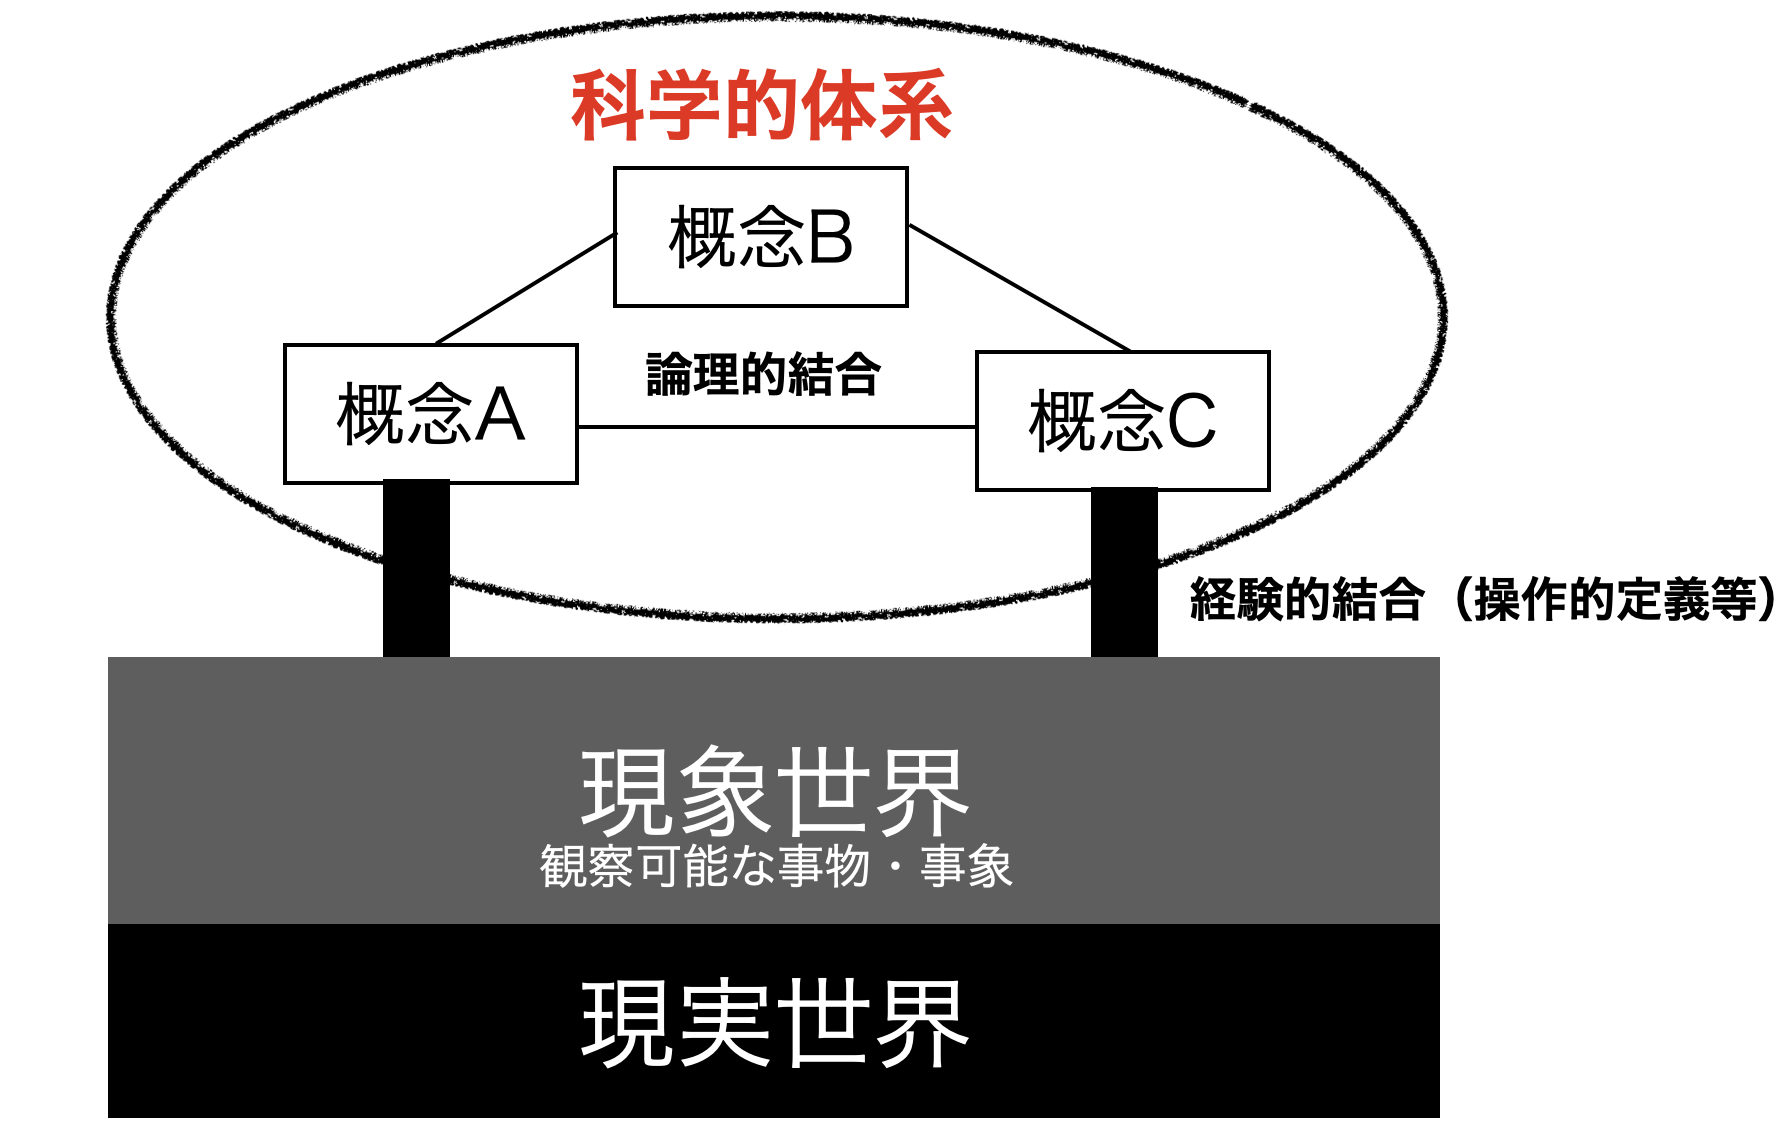
\includegraphics[keepaspectratio,width=0.8\linewidth]{../images/03_constructs.png}
	\caption{構成概念}
	\label{construct_concepts}
\end{figure}

構成概念同士はいろいろな説明の仕方で結びつきます。科学的体系の中では，理論的・論理的な結びつき方をします。この現象・現実のレベルから上に行っているということは，もう客観的に見て分かるものではなくて，抽象的な世界に入っているわけです。その中で，別の概念Bというやつが，理論的な結びつきだけで構成されている。こういうことも考えられるんですね。こちらも抽象の理論の世界です。

少し浮世離れしたところに，構成概念というのはあるんです。ただ，構成概念というのを現象・現実に対応する，何か具体的なものに接地しておかないといけない。そうしないと空中戦になって，何を言ってるかわからなくなる。接地のさせ方は，操作的定義と言われたりします。抽象概念に裏支えられている，さらに高度な概念なんかになると，もはや直接現象とか現実に根ざしていない分，よっぽどしっかりしておかないといけない。この理論の世界，抽象の世界で論理的に縛り付けておかないと，抽象的すぎてふわふわしてしまうわけですよ。だから我々は専門用語を使って話をするんです。なんでそういった用語がいるかっていうと，抽象度が上がれば上がるほど，もうなんか現実に足がついてない。それはどこの何の話をしてるんですか，というようなことになるからです。

マービン・ミンスキーという人\footnote{マービン・リー・ミンスキー(Marvin Lee Minsky，1927年8月9日 - 2016年1月24日)は，アメリカ合衆国のコンピュータ科学者であり，認知科学者。専門は人工知能 (AI) であり，マサチューセッツ工科大学の人工知能研究所の創設者の1人。初期の人工知能研究を行い，人工知能や哲学に関する著書でも知られ，「人工知能の父」と呼ばれる。(Wikipediaより)}が，昔「心の社会」という分厚い本を書いたんです\parencite{minsky1990}。それは面白いので読んでもらいたいんですけど，それをさらに分かりやすく書いたと本人が言っている，「ミンスキー博士の脳の探検」っていう本もあるんですよ\parencite{minsky2009}。よかったらそれを読んでみてください。冒頭のところが面白くて。色々言葉を使って心の動きみたいなのを，いろんな人が表現してるけど，それは何も指し示してないですよ，っていうようなことを言います。ミンスキー博士は心理学を攻撃してるわけではないんですが，我々が普段使う心に関する用語みたいなのを見てみると，ほとんどが``スーツケースワード''だっていうんです。その言葉の中に何でも入っちゃう，その言葉でまとめておいたら，理屈が通った気がする。でも分かったような気になってるだけで，そういうふうなまとめ方したかった心のことは分かんないですよ。社会のことは分かんないですよ，っていうようなことを「脳の探検」の冒頭のところで，すごく警句を述べてらっしゃいます。僕も本当にそれはそうだと思います。

心理学をやっていますと，色々流行りの言葉みたいなのがありまして，特に応用的なシーンが多いんですが，流行り言葉で言いますと，最近の一番の流行りはMBTI\footnote{Myers-Briggs type indicatorの略。心理学的な個人の選好を簡単なチェックリストで分類できるもの。ただし理論的なMBTIとそれを専門に扱っている心理学者，および日本で流行しているWebテストはそれぞれ別物で，学術的な裏付けがないものの心理学的な何かとして，2023年ごろから流行しています。}ですかね。あれはもう僕らにとっては，何のこっちゃ分からないんですが，そういうやつです。とかちょっと前だったら，HSP\footnote{Highly Sensitive Person，「とても敏感な人」の意味の用語。心理学や医学における臨床的・病的なケースではなくても，自分はそうかもしれないという妙な共感を呼びやすいワードで，2018年ごろから流行しています。}というのがありましたね。ハイセンシティブパーソンですか。他人のことを気にしすぎる私たちとか，っていうやつですが，ああいうのがネットだとか世間では，あの人HSPなんじゃないとか，MBTIというと私はなんとかなんとかで，とかっていうのって，ものすごく流行るんですけれども，流行ってはいるんですけれども，心理学業界ではなかなか，どちらかというと，眉唾ものの代表格です\footnote{変な心理学が流行りやすい理由はいくつかあって，科学を標榜しているからしっかりしていると思われやすいこと，マスコミやネットを通じて流行しやすい「心理テスト」というツールで話題になりやすいこと，心理学者の中にも売名目的でそのような活動に加担する人がいること，などが挙げられます。心理学は真面目にやってるんですよ，ということを言うための本\parencite{Keith2016}もあるぐらい，専門家は辟易しているんですが，皆さんは努努踊らされないでくださいね。}。

これも前回言いました。例えばHSP。私HSPかもしれないから，これを心理学の勉強ではっきりさせたい，とおもって心理学を志した人は，実際大学に入って研究しようとすると困ると思うんです。専門家に聞いたら，それ何？って言われちゃう。心理学者は全員，そういうのは眉唾ものだと思っていたりするわけですから。新しい構成概念を作るんであれば，従来の構成概念で説明できなかったことが説明できる成分があって，かつ，それでなければ言い表せないようなものがないといけない。さらに言うと，できればそれが具体的な現象，現実に根付いていないと，やっぱりそれがわかったことにはならないわけですので。HSPを提唱するのはいいですが，従来の心理学で言うところの性格だとか，対人恐怖症だとか，自尊心，自己愛傾向といった言葉と，どこが同じでどこが違うのか，っていうことを詰めていかないといけないんです。これは，我々が現実現象に足はつけてはいながら，かなり抽象的な世界で話をしようとしているからです。ここが崩れると何の話もできないというわけです。

\subsection{人文社会科学における客観性}

ちなみに，心理学あるいは人文社会科学における客観的なもののあり方というのは，どういうふうにして考えるかと言いますと，カントが言ったように対象はもう認識に従うわけですから，客観的になんとかっていうのは言えないわけですね。

例えば，ここに木があります。私がそれを見ています。見ていますというと，これは私が見ているわけですから，私の主観なわけです。いやいや，他の誰が見たがってあそこに木があるじゃない，りんごがあるじゃないと言ったとしても，あくまでもそれは人の主観にしかなってないわけで，主観がいっぱい集まったから客観になるというような，そんな単純な話ではない。客観というのは何かというと，自分が見ているではなくて，見ている人を見て，見えている姿が客観的である，というだけ。つまり，AさんはBさんが見ている事実を支持することはできます。そうすると，客観的に見て，あなたはあれを見ていますよっていう，自分が見ているではなくて，他の人がそれを観察している，見ているっていうことをサポートしてあげることができたら，初めてこの人は客観的に主観を持っているねって言えてるわけです。で，Bさんもあなたもこれを見ていますねというふうなことをサポートしてあげることによって，あなたが木を見ている，あなたは木が見えているというのですねっていうのを，Aさんにとって客観的にサポートしてあげることができるわけです。だから，客観的にここに木が存在するということを言うためには，少なくともこの私がこの人の主観をサポートし，この人がこの主観をサポートし合う必要がある。そうすると，少なくとも2人にとっては，客観的に木が見えているという現象が存在する。こういう形で持って，客観性というのを担保するしかないはずなわけです。なので，人間科学，人文科学における客観性のあり方というのは，こうやって互いが互いの主観をサポートし合いますよっていうところにベースがある。物自体の世界とか，ニュートン\index[nameidx]{にゅーとん@ニュートン}が考えた絶対空間，絶対時間の中にポーンと木がある，我々が見ていなくとも客観的に木が存在するとかっていうのはもう言えない。客観的に何かが存在するというのは，くどいようですが，それぞれの主観を相互にサポートし合っていること，主観を互いに支え合っているということに依存している。つまり，この人の客観的なサポートを通じて，AがBの主観をサポートし，BがAの主観をサポートすることで，ここに像が出来上がる，客観的に像があると言えるようになるわけです。これが人文社会科学が考えるべき客観の姿なのです(fig.\ref{objective_subject})。

\begin{figure}[ht]
	\centering
	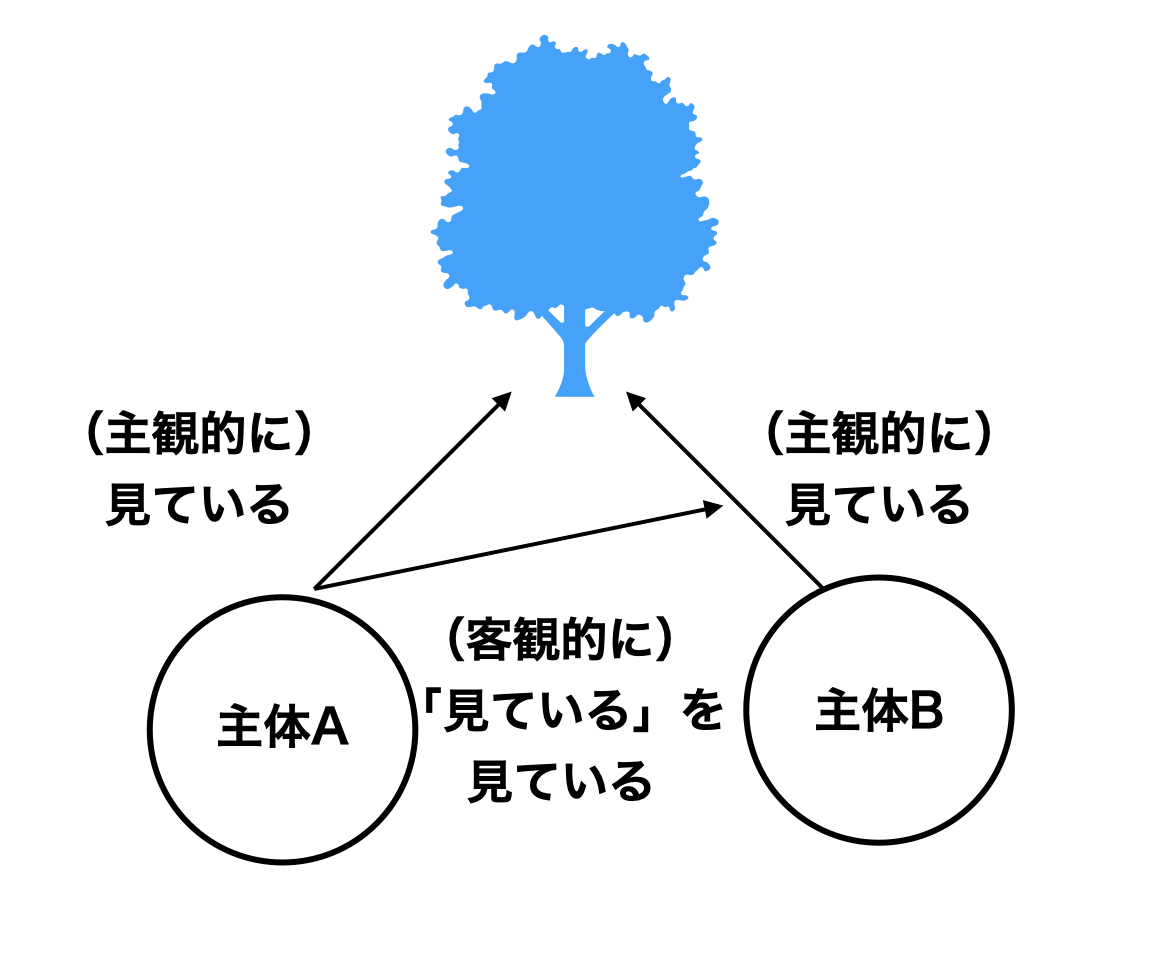
\includegraphics[keepaspectratio,width=0.8\linewidth]{../images/03_subject_object.png}
	\caption{主観を支え合う}
	\label{objective_subject}
\end{figure}

\subsection{実在の社会的構築}
実は，勘の良い人はお気づきのように，これで成立するのであれば，実際はここに木がなくてもいいんです。自然科学的にはどうか知りませんが，少なくとも人間のサイエンスとしては，ここに木がなくてもいいです。例えば，今日は5，6人にですね，僕がね，ここにね，小さい妖精さんがいますっていう話をしたとします。ここに小さい妖精さんがいますよ，妖精さんがいますよって言いながら，今日は話をしたとします。僕がすごくこう熱を持って喋って，皆さんがもう仕方がない，小杉の言うことに乗ってやろうと思って，その妖精さんはどんなのですか，その妖精さんは可愛いですねとかっていいながら，みんなでその見えないものを介して，この見えないものの存在を全員がサポートし合うのであれば，この世界の中にはそういった小さいおじさん妖怪が実在すると考えても，構わないでしょうよね。別に全員が一つの同じ対象をサポートし合っているのであれば，物理的な物体である必要はないわけです(fig.\ref{socialReality})。
\begin{figure}[ht]
	\centering
	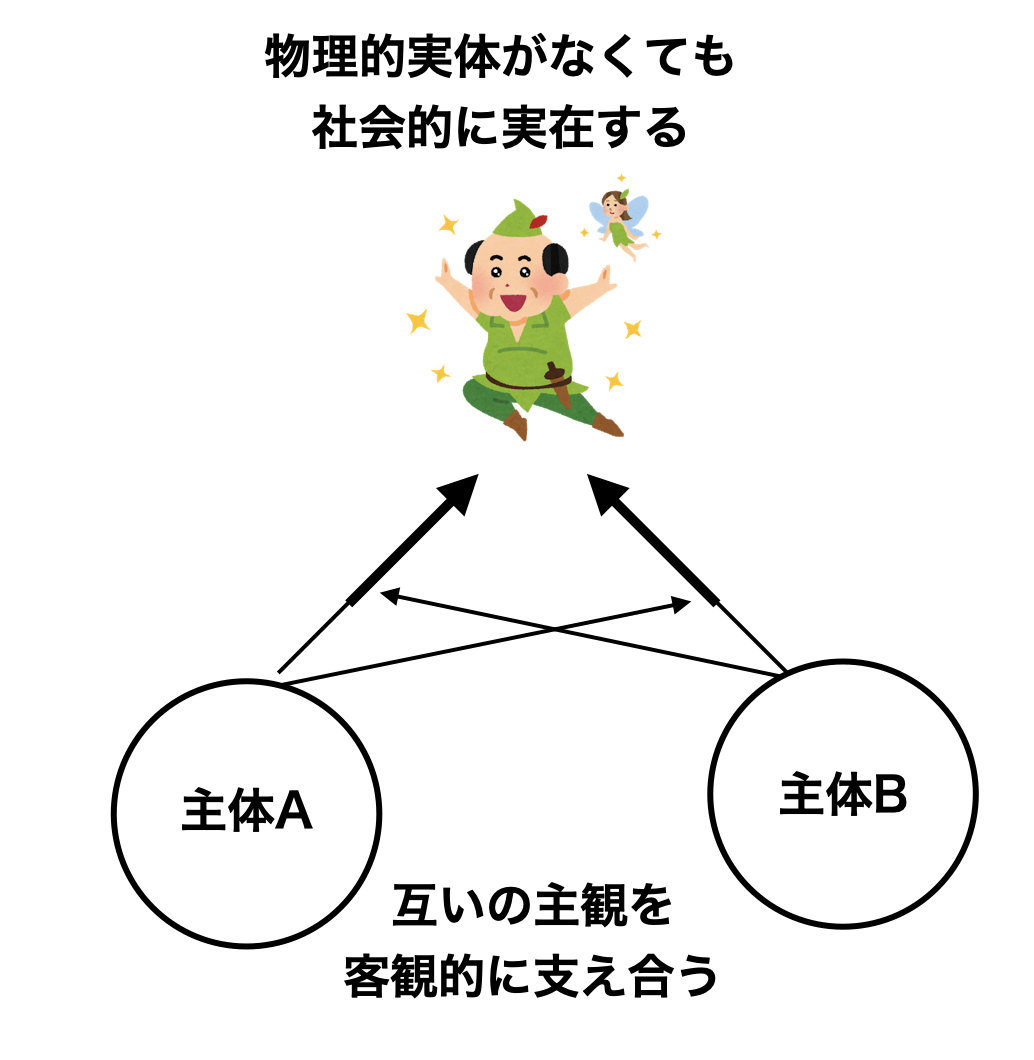
\includegraphics[keepaspectratio,width=0.8\linewidth]{../images/03_socialReality.png}
	\caption{小さい妖精さんは社会的時に実在する}
	\label{socialReality}
\end{figure}

社会心理学\index[termidx]{しゃかいしんりがく@社会心理学}だとか心理学が成立しているのは，恐らく今みたいな感じで，みんながそれがあると思って振る舞っているからです。だから，自分の感覚としては社会があるかどうかはわからないが，社会があると言っている人を客観的に観察することはできるし，私がそのみんなが考えている社会とやらについて語ることをみんなが客観的に確認することができるので，全員が互いに他者の主観をサポートし合って，その実在の存在を見つけている。これが人文社会科学における客観性の持ち方，対象の理解の仕方というのではないでしょうか。僕なんかはそういうものなんだろうなと思っていますが，皆さんも考えてみてください。

このことを\textcite{fujisawaCore}や\textcite{fujisawaIntro}では，\textbf{リアリティールプ}と呼んでいます\footnote{著者の藤澤等(1948年2月20日生まれ)は，関西大学社会学部，長崎シーボルト大学国際情報学部で教鞭をとったひとで，筆者の学部時代のゼミ指導教員であり，社会心理学\index[termidx]{しゃかいしんりがく@社会心理学}，心理統計学の考え方の基礎を方向づけた人です。}。Aという人の持っている主観で客観的にBの存在をサポートする。BはBで主観的にAの存在をサポートすることで，このお互いが主観と客観のループを形成することによって，初めて両者ともに客観的な何か，両者で表現できる客観的な何かというのが成立するよ，ということを説明しています(fig.\ref{realityLoop})。
\begin{figure}[ht]
	\centering
	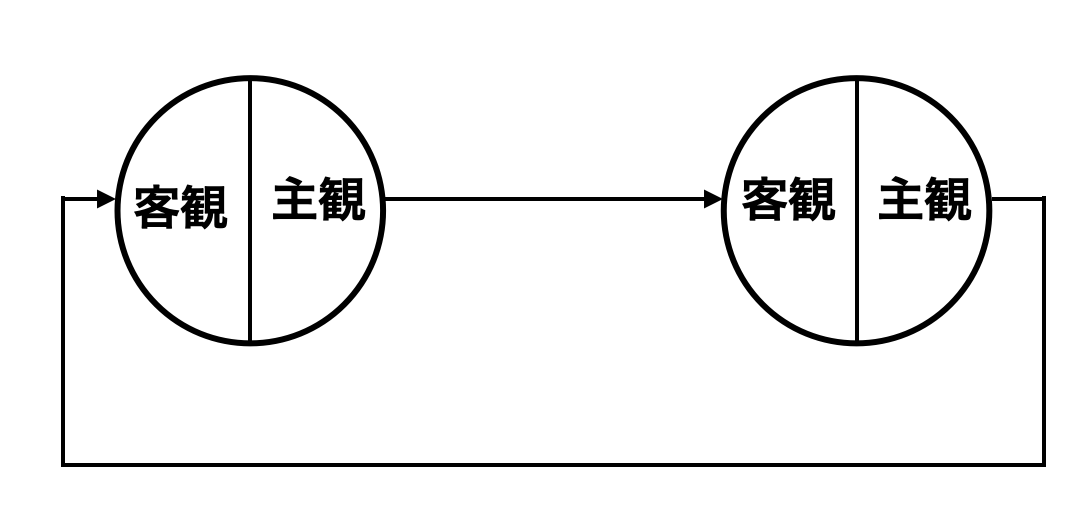
\includegraphics[keepaspectratio,width=0.7\linewidth]{../images/03_reality_roop.png}
	\caption{リアリティールプ}
	\label{realityLoop}
\end{figure}

さて，何か変な話をしているような気もしてきましたが，いかがでしょうか。主観と客観というけれども，客観的に存在するという話でサイエンスというのはやってきてたわけです。自然科学はバリバリに客観的なもので話を作っている。サイエンスってそういうものじゃないんですかと思われるかもしれませんけれども，少なくとも人文社会科学においては，実体というより実在，本当にそこにみんながあると思っているものを研究対象にする。みんながこういう現象をこれと名付けましょうって，全員がその存在をサポートし合う抽象的なものをサイエンスする。そういう抽象的な構成概念であったとしても，社会的には実在し得るわけです。社会心理学\index[termidx]{しゃかいしんりがく@社会心理学}が研究すべき対象の「社会」というのは，みんなが信じているけれども，最初から物理的な実体がないものですから，全員がそれをいかに信じられるかというところに立脚するしかないような気がします。

そんなものがサイエンスなのか？それこそ今日だったら十人もここにいないんですから，僕らがここに妖精さんがいる，キャッキャッキャーって言ってたとしても，他の人から見たら怪しいな，あの授業何やってるんだとなるでしょうね，きっと。そうだとは思うんですけれども，もしみんなが本当にそこにそれがある，そういうものだと理解したら，それはこの社会では成立するじゃないかというようなことを人文社会科学は考えていかないといけないわけです。だからあながち社会心理学\index[termidx]{しゃかいしんりがく@社会心理学}も遊びでやってるんじゃないよというようなことが言いたい。ただ気をつけないといけないのは言葉遊びになりうる，全部スーツケースワードになりうる可能性があるという点です。みんながHSPっぽいよねとかMBTIっぽいよねといった，曖昧な考えで持って，専門的でない用語で非常に庶民的な，一般的な概念みたいなので説明して納得するというようなものが，そのままサイエンスになりうるかというと，それはおそらくそうはならない。それはなぜかというと，その界隈だけで通じる話題とかっていうのはやっぱり広まり方が弱いからです。というような話をこの後したいと思います。

\section*{いんたーみっしょん；読書案内}

ちょっと休憩。息抜きがてら，今日私が持ってきた本についてちょっとご紹介します。今日は別に，この本の内容について話すわけではないんですが。もし本の内容に触れた時は参考文献として，講義録に必ず付けておきますね。せっかくだから，知っておいてもらいたいというか，ご自身で学ぶときの資料としてね。いろいろ書いてある本を持ってきております。

一つは，戸田山先生の『科学哲学の冒険』という本\parencite{todayama2005}です。さっき僕が，哲学者が「心理学者って，構成概念構成概念ってこだわるんですね」と言って驚いたと言いましたが，この本を書いたのがその哲学者の方です。この方は科学哲学者で，もしかすると『論文の教室』\parencite{Todayama2022}でご存知の方もいるかもしれません。また，『論理学をつくる』という本\parencite{Todayama2000}も書いています。『科学哲学の冒険』は，科学がどうして成立するのかについて書いてある本で，今日の話とも少し平行するところがあるかなと思います。

今日，どれくらい触れるかどうかわかりませんが，この後，少し現象学について話をする予定です。
今日は『アナトミア社会心理学\index[termidx]{しゃかいしんりがく@社会心理学}』という本\parencite{anatomia}の第3章，いや，第4章の内容なんですが，社会思想哲学についての話がメインです。社会心理学\index[termidx]{しゃかいしんりがく@社会心理学}を勉強するにあたって，なんでそんな思想とか哲学の話を聞かされるんだと思われるかもしれません。しかし，今回や次回で，皆さんに感じてもらいたいのは「20世紀初頭の科学万歳感」なんです。

「感じてもらいたい」と言いましたが，僕自身は1975年生まれなので，当時を知っているわけではありません。しかし，いろいろな資料を見ていくと，どうも20世紀初頭には「科学って素晴らしい」という世界的なノリがあったように思います。それはもう想像するしかないのですが，みんなが異常に科学的なことについて考えたり，行動したりしている時代だったのです。そして，「科学は良いものだ」と一辺倒で話が進んでいた時代でした。

その理由の一つには，物理学が大成功したことがあります。実際，そのおかげで生活が豊かになり，それまでの生き方や考え方が大きく変わりました。世界のあり方だけでなく，それに伴う人間の考え方も変わっていきます。そういう思想的な展開は，リーダー格の人材が現れると言うか，いくつかの人々が牽引していくのです。

例えば，ガリレオ\index[nameidx]{がりれお@ガリレオ}やニュートン\index[nameidx]{にゅーとん@ニュートン}が近代科学をぐっと引っ張り，デカルト\index[nameidx]{でかると@デカルト}が科学の入り口を開き，カントが「世界の認識とは何か」という哲学的な問いをぐっと深く追求しました。それに影響されて，いろんな学問，学術，派閥，哲学，思想的な流派が生まれました。

カントの時代までは，哲学といえば一言で済ませることができましたが，20世紀前後の頃には「現代思想」と言われることが多くなりました。なぜなら，いろんなジャンルの人々がその話をするようになったからです。哲学ばかりをやっていた人もいれば，哲学の中に言語学や論理学を取り入れる人も出てきました。また，人類学が考え方に影響を与えることもあったのです。

20世紀の科学の発展や「科学ってすごいな」という世界の裏には，「人間の世界ってすごいな」というような，いろんな発見があったんじゃないかな。その流れで，社会科学や人文社会科学，そして社会心理学\index[termidx]{しゃかいしんりがく@社会心理学}が，学問として発展してきたわけです。そういった背景を無視して，「社会心理学\index[termidx]{しゃかいしんりがく@社会心理学}は科学です。統計でこれだけのことがわかります」とだけ言っても，何かが足りないように感じます。

そういう意味で，面白い本をいくつか紹介しておきます。『そうだったのか現代思想』という本\parencite{kosakashuhei2000}は，とてもわかりやすく，熱っぽく書かれています。登場する人物は，ニーチェ\index[nameidx]{にーちぇ@ニーチェ}，フロイト，ハイデガー，ソシュール，サルトル，ドゥルーズ\index[nameidx]{どぅるーず@ドゥルーズ}，フーコーなどです。冒頭ではニーチェ\index[nameidx]{にーちぇ@ニーチェ}について話しています。ニーチェ\index[nameidx]{にーちぇ@ニーチェ}は1900年に亡くなったのですが，とにかく「ニーチェ\index[nameidx]{にーちぇ@ニーチェ}，すごい」という言葉で始まります。読んでいただければ，何がすごいのかがわかると思います。

また，『史上最強の哲学入門』という本\parencite{yamucha2015}もおすすめです。ちょっとカジュアルな表紙で，拍子だけ見ると気軽に手に取れりにくい本ですが，内容は比較的わかりやすく書かれています。

僕は社会心理学\index[termidx]{しゃかいしんりがく@社会心理学}や心理統計を専門にしていますから，哲学や科学史を専門にしている人から見れば，「何を生ぬるいことを言っているんだ」と思われるかもしれません。しかし，こうした知識を持って社会心理学\index[termidx]{しゃかいしんりがく@社会心理学}を見るか見ないかで，見え方が変わることもあるかもしれませんので，ちょっとした紹介でした。

\section{科学コミュニティの構造}
\subsection{パラダイム論と現代科学}
さて，本筋に戻りましょう。皆が信じていることが実在すると考えられる理由や，サイエンスの世界が必ずしも正しいことだけを追求しているわけではないという視点は，科学哲学の一部です。トーマス・クーンが書いた「科学革命の構造」という本\parencite{ThomasKuhn1962}を読むと，科学が発展する過程は一筋縄ではいかないことがよくわかります。

``通常科学''というのは，現在広く認められている科学的な考え方や理論のことを指します。しかし，その理論に矛盾する事象が出てくることがあります。例えば，ニュートン\index[nameidx]{にゅーとん@ニュートン}が提唱した絶対空間や絶対時間という考え方に疑問を持ったアインシュタイン\index[nameidx]{あいんしゅたいん@アインシュタイン}は，光の速度で移動しながら，光を見たらどうなるかという視点から新たな理論を提唱しました。それが相対性理論\index[termidx]{そうたいせいりろん@相対性理論}です。しかし，その理論が発表された当初は，ほとんどの人に理解されませんでした。その新しい理論が異端とされ，否定されることもあります。しかし，そうした議論の中で新しい科学が生まれるのです。

「どうも通常科学というのがこれ以上維持できないぞ」という状況が生じたとき，一気に考え方が大きく変わる。これをパラダイムシフトと言います。このようなことをトーマス・クーン\footnote{トーマス・サミュエル・クーン(Thomas Samuel Kuhn，1922年7月18日 - 1996年6月17日)は，アメリカ合衆国の哲学者，科学者。専門は科学史及び科学哲学。(Wikipediaより)}は『科学革命の構造』という話の中で述べました。それまで，科学とは真実性のゲームだと考えられていました。つまり，何が正しいか，または正しくないかという問いが中心でした。正しいと思われるものは，それが偉い人が言ったことであるとか，お金持ちが言ったことであるとかいう理由からではなく，それが正しいか正しくないかだけに基づいて評価されるべきです。そうすれば，正しいことを言うことで必ず前に進めるはずです。これは普通の人が考えることですが，トーマス・クーンによると，科学界は必ずしもそうなっていないぞ，と。科学コミュニティがその変化を受け入れるようなパラダイムシフトが生じないと，新しすぎる考え方は受け入れられないというのです。もし新しい考え方が受け入れられれば，それが新しいスタンダード，新しい通常科学の状態になります。しかし，それを変えるためには，一部が異端とみなされるという状況を乗り越えなければなりません。その中でいくつかは次への扉を開く可能性があると言います。つまり，真実かどうかということだけでは，科学は進みません。これらのことをトーマス・クーンは「科学革命の構造」で語っています。

\subsection{現象学的理解}
これと似たようなことが，現代思想の話の中でもいろいろ出てきます。例えば，この本，「現象学は思考の原理である」という本\parencite{TakedaSeiji}があります。この本は現象学の本で，一部と二部に分かれています。二部は現象学についての詳しい話で，一部はその前の話です。つまり，物事を考えるためには，現象学的な発想しかないという話です。現象学というのを，僕が一言で説明するのは難しいので，このテキストを読んでいただければと思います。しかし，少なくとも言えるのは，デカルト\index[nameidx]{でかると@デカルト}風の発想で，今まで考えていたことを一旦忘れて，確実に分かっていること，見えていることだけから判断していこうというのが，現象学的な考え方だということですね。

この本で言いっているのは，真実かどうかということだけを持って人とコミュニケーションをすると，それは喧嘩にしかならないということです。真実かどうかということがゴールにあるなら，答えは一方に決まってしまいます。つまり，真か偽かと判断できてしまうからです。その結果，世界のあり方はどちらかになります。ならなかった方は偽物，まちがいです。「本当か嘘か」という議論だけでは，絶対に本当派と嘘派に分かれてしまい，しかもそれはどちらかが勝つまで結論がつかないのです。

科学のあり方，あるいは実際の世の中のあり方というのは，全ての前提条件や全ての状況が分かっているわけではありません。我々が見えている世界の中でのもっともらしさが，どの程度あるかというのが問題なのです。例えば，マックスウェルのデモンのように，全てが分かっていて，本当の状態か嘘の状態かといったこともあるかもしれません。しかし，我々が世界を見るというのは，神の視点のようなものはどこにもないということです。少なくともニーチェ\index[nameidx]{にーちぇ@ニーチェ}が「神は死んだ」と言ってから神はいなくなったので\footnote{念のため言っておくと，これは冗談です。}，神の視点というのは存在しません。

私たちは自分自身の認識の世界の延長線上で生きています。世の中のこと全てを知っている，全てを書いているものなんて存在しないとなると，自分が最も信憑性のあると思えるものは，自分の学んだ範囲でしかないのです。つまり，コミュニケーションが成立するとか，人と話をするときにできるのは，私が持つ，今視界に入っているような，世界の見方を元にしています。「世界はこのようなものだ」と仮定しているんです。その前提でいえば，ある考え方Aが最も妥当なものと思える，とはいえます。その中で，信憑性がどの程度あるのかという問いや，全てが私という主観的な視点からしか物事を語れないという事実が，現象学の話のスタートなのです。

現象学というのは，自分の感覚を，客観的にどう見えているか，神様がどう見ているか，一般的にどうなっているかといった視点から語らずに，そうした観点を一旦横に置いて考える方法です\footnote{横に置いておくことを現象学用語で，エポケー\index[termidx]{えぽけー@エポケー}といいます。}。自分がどう考えているか，どう見えているかという観点，この見えている世界からしか私たちは語れないのです。だから，この世界の中で，「これが最も妥当でしょう」というような話をするのです。皆さんの中にも，皆さんなりの世界の見え方があるでしょう。幸いなことに，ほとんどの場合，「例えば，ここにカメラがありますね」という認識は\footnote{授業をしていた東京大学法文大2教室には，教壇の前にウェブカメラがありました。オンライン授業用のものでしょうね，きっと。}，みんなにとってもっともらしいものとして，実在するものとして認識されるため，会話が成立します。しかし，「ここにカメラなんてない」という人がいたとしたら，その人の視点，その人の認識する世界によっては，それが事実なのかもしれません。

このような点から，この本では現象学を「思考の原理である」，「物事を考える時の原理，マナーである」と説明しています。「ああ，見てごらん，ここにカメラがあるよ。あなたが間違っています」という話をしてもいいですよ，もちろん。でもその人が本当にカメラを見えていないとか，理解できていないというのであれば，それは存在しないことと同じです。だから，正しいか間違っているかで議論しても，勝つか負けるかで決めることになるし，その根拠は「超自然的な客観」みたいなものを想定しないことには成立しない。

我々ができるコミュニケーションや理解というのは，どの程度の信憑性を担保できるかという問いに直結します。例えば，「私は科学的にここにカメラがあることを説明します」と言っても，それを説明する方法は多種多様です。もしかすると，「私は宗教的にここにカメラがあることを説明したいと思います」と言えるかもしれません。神様がカメラを作ったという話を，理論的な体系で説明できるかもしれません。皆さんがその信者であれば，神様がここにカメラを作ったという理論が，信憑性が高いと思えるかもしれません。

もし，それがこの世界の多数派の意見だったら，おそらくその方が社会的な実在性が強いでしょう。だから，この世界の中ではそれがより正しいというしかありません。それが思考のマナーだと，この本は言っています。この考え方は，先程のトーマス・クーンのパラダイム論\index[termidx]{ぱらだいむろん@パラダイム論}とほとんど同じだと思います。

科学者が，「科学はこういうものだ」という考え方をすると，そのバックグラウンドの中で，その手続きが正しいと思っている人々の集まりで，そのコミュニティの中ではそれが正しいとされるでしょう。それを信じているなら，そのコミュニティの中ではそれが科学的で，それが正しいということになります。「いやいや，そんなの科学でもなんでもないよ。間違ってるよ」という話をすると，正しいか間違っているかの議論になります。

現象学的な視点から，「客観的に正しい」って何なのかという話になると，神様目線の「客観的に正しい」を再度定義しなければならないでしょう。それは別の話になってくるのですが，少なくとも現代に生きる我々にとって「正しい」とは何かを考える必要があります。

真実度でなくなるとすれば，自分たちが考えているこの世界のフレームワークの中で，信憑性の高さが重要だということになります。例えば，何か奇抜な宗教やカルト的な宗教を信じていると，その宗教の中では信憑性は高いかもしれませんが，全世界に対する普遍性は低いです。あなたにとってはそうかもしれませんが，その考え方が世界中で通用するかというと，そうではないと言えます。

つまり，サイエンスとは，普遍性の高い科学的コミュニティのトレーニングを受けた人々の，共通理解が作り出す世界ではないでしょうか。トーマス・クーンが言うパラダイム論\index[termidx]{ぱらだいむろん@パラダイム論}とは，そういうことだと思います。

\subsection{社会心理学も科学ですよ}

「正しいか，正しくないか」ということについては，カール・ポパーの主張によれば，「反証可能性」が重要です。正しいと証明することはできませんが，科学を進めていく中で，「正しいとするとこうなるはず」ということが発見できるでしょう。しかし，この方法では，科学，その前提，仮定，モデル，研究方針が正しいかどうかはわかりません。ただ反証を探す方法があるというのが，科学の存在理由です。これが，ポパーが主張する反証可能性であり，現代の科学のあり方です。少々話が行ったり来たりしているように感じるかもしれませんが，私は社会心理学\index[termidx]{しゃかいしんりがく@社会心理学}は，人文科学的な存在，客観性を基にした，多くの人が科学的だと信じている方法によって運用されている人文社会科学の一つであり，社会心理学\index[termidx]{しゃかいしんりがく@社会心理学}が間違っていないと言いたいのです。

そのために，これだけ回りくどい話をしています。科学とは客観性が重要だと言いつつ，自然科学であってもパラダイムから逃れることはできません。科学として残ることができる，科学として述べられることは，主観性を排除することです。現代的な表現を使えば，反証可能性が保証されているものであれば，それを科学と呼ぶことができるところまで，科学論は進んできました。

カルト的な宗教で理論的に説明してもいいんですが，そこに反証可能性がなければ，科学のグループには入れてもらえません。「なぜそう言うのかというと，教祖がそう言ったからです。教祖が正しいか間違っているかは検証できません」と言われたら，少なくともそれは科学ではありません。しかし，そのコミュニティ内の信憑性は，科学のそれとは遜色がないですよ，ということは考えておいた方がいい。

言葉を変えれば，科学とは，一つの宗教にすぎないんです。そう言うと言葉が悪いかもしれませんが，普遍性が高く，多くの人が納得しがちな考え方の総体のひとつが科学だと言えるでしょう。サイエンスっていうのは物理学的で，感的で予測と制御するためだけのものです，と言い切ってしまうほど客観的なものでもないんではないでしょうか。科学というのもある程度相対化して捉え，かなり普遍性が高いもぐらいと考えて，その視点で人文社会科学の存在をどこかに位置付けると言うか，地に足をつける，，認めてあげることはできるんではないかなと思っているわけです。いかがでしょう？社会心理学\index[termidx]{しゃかいしんりがく@社会心理学}は科学なのか，あんなもん遊びじゃないのって言われた時に，これで多少は反論できるでしょうか。

ただ，社会心理学\index[termidx]{しゃかいしんりがく@社会心理学}の中でも，その考え方が間違っている場合があります。社会心理学\index[termidx]{しゃかいしんりがく@社会心理学}コミュニティが，第1回の授業で言ったように，狭くて，身内同士が相互に参照しあってしているだけの状態にあると危険です。つまり，お互いがお互いの論文を参照し合い，社会心理学\index[termidx]{しゃかいしんりがく@社会心理学}会に入って，社会心理学\index[termidx]{しゃかいしんりがく@社会心理学}的な発表をした人が社会心理学\index[termidx]{しゃかいしんりがく@社会心理学}者であるというような，自家発電的で閉鎖的な定義しかできないのが社会心理学\index[termidx]{しゃかいしんりがく@社会心理学}かと言われると，それはおそらく困るわけです。

その辺りは，きちんとチェックする必要があるでしょう。しかし，我々がやっていることは一つの考え方に過ぎず，絶対不変のものではないという視点を持つことが，おそらく必要ではないかと思います。『現象学は<思考の原理>である』という本には，今言ったように，「正しいか正しくないかで喧嘩する意味はない」ということが書かれています。この本は，もちろん僕の説明よりも分かりやすく，丁寧に書かれていますので，ぜひ読んでみてください。

\section{時代背景；知の相対化の道のり}

論理実証主義\index[termidx]{ろんりじっしょうしゅぎ@論理実証主義}の話もしておきたいですね。どうしようかな。皆さんもお疲れと思いますが。

ちょっと喋り疲れたので，投影資料を使ってお話ししますね。これは昔，私が学生の頃に読書会用に作った資料なのでお見せするのが恥ずかしいんですが。
\begin{figure}[ht]
	\centering
	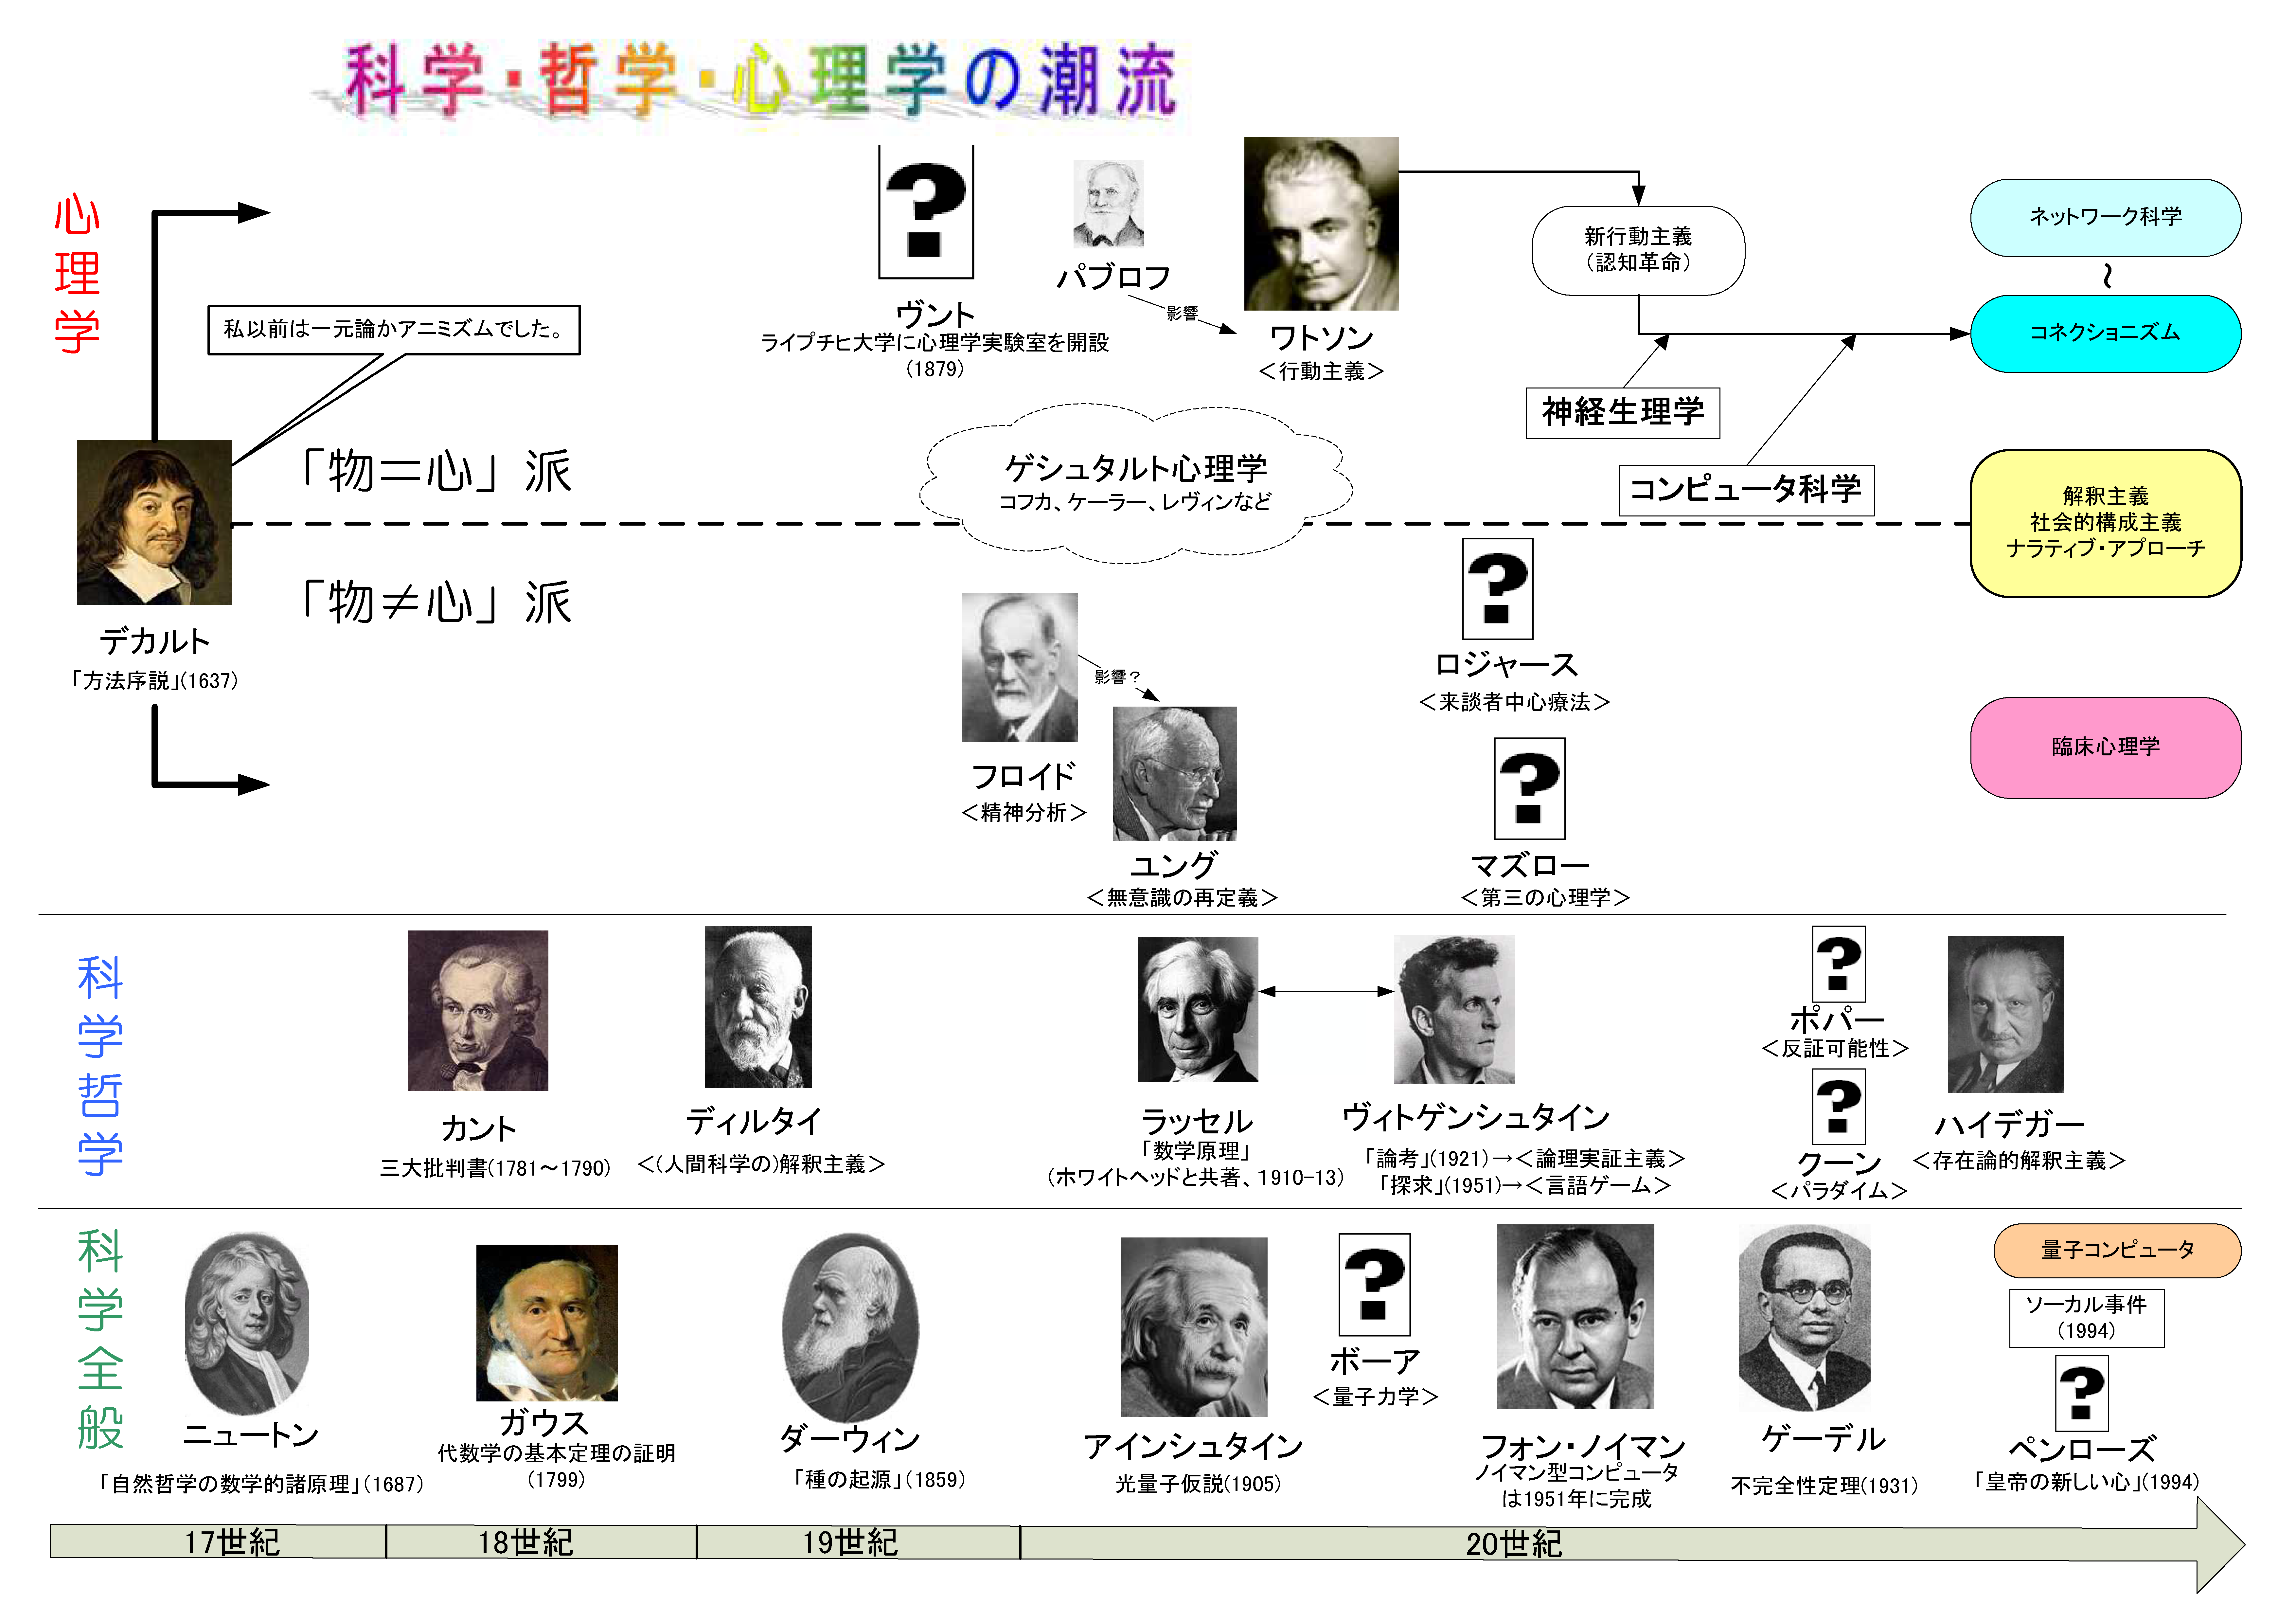
\includegraphics[keepaspectratio,width=1\linewidth]{../images/03_modern_philosophy.png}
	\caption{科学，哲学，心理学の潮流}
	\label{modern_philosophy}
\end{figure}


ここ何回かの話を図示したらこんな感じです(fig.\ref{modern_philosophy})。この授業のどこかで出てきている研究者の顔，名前がはいってます。

\subsection{心理学の潮流}
まずスタートはデカルト\index[nameidx]{でかると@デカルト}にしました。方法論的懐疑が1637年。ここで心は物なのか，心と物質というのは一緒なのか，違うのか，みたいな発想が出てきます。いやいや，心は心の世界があるよっていう考え方もきっとあるでしょうし，心も物理学のように，物のように扱って研究もできるでしょうという幅広い視点もあるでしょう。それで大きくデカルト\index[nameidx]{でかると@デカルト}をスタートにして上下に分けてみました。ちなみにこの図は左から順番に時代の変遷を辿っていますから，大体17世紀から20世紀までの流れがあるわけですけれども，これで見ていただきますと，1879年にヴント\index[nameidx]{ゔんと@ヴント}がライプチヒ大学に実験室を作ってます。この時は実験室を作っているというのですけれども，ヴント\index[nameidx]{ゔんと@ヴント}が取った手法が内観法\index[termidx]{ないかんほう@内観法}というやつで，あなたの今の心の状態はどんなですか，みたいなことを聞いて答えさせるようなやり方だったわけです。そこで心が分かるのか，実験室という意味で哲学からは袂を分かちましたと言うんですが，どうにも怪しい。ということで，ロシアの生理学者パブロフ\index[nameidx]{ぱぶろふ@パブロフ}に影響を受けたワトソン\index[nameidx]{わとそん@ワトソン}先生が出てくるわけです。20世紀の真ん中あたりですね。1913年でしたっけ，行動主義宣言がでてきます。その後，認知主義に変わるという話をしましたね。S-O-R，中の有機体Organizationの中身も考えましょうという話が出てきます。ただ，それには神経生理学だとかコンピュータ科学の影響みたいなのが多分に入ってきています。その矢印の延長線上にコネクショニズム，ネットワーク科学\index[termidx]{ねっとわーくかがく@ネットワーク科学}に行き着きます。当世風には，AIとか機械学習と言った方がいいでしょうか。

ただし，それに対抗する考え方として，位置づけがすごく困るんですけど，行動主義宣言に対するアンチテーゼとして，心理学だとか無意識心理学，フロイド\index[nameidx]{ふろいど@フロイド}一派みたいなのは考えておかないわけにはいきません。この辺については次回もちょっとゆっくりお話できるかなと思います。フロイド\index[nameidx]{ふろいど@フロイド}先生が活躍したのはちょうど1900年になった頃ですね。図の真ん中に，フロイド\index[nameidx]{ふろいど@フロイド}とかユング\index[nameidx]{ゆんぐ@ユング}というのが出てます。こういう書き方をしたらものすごく主流派な気もしますけど，フロイド\index[nameidx]{ふろいど@フロイド}とかがやってた精神分析\index[termidx]{せいしんぶんせき@精神分析}っていうのが，さっきも言ったように，いわゆるサイエンスと，人文社会科学的なサイエンスの営み，自然科学的なサイエンスと，人文社会科学的なサイエンスと，そのどれでもない第3の営みみたいなことが精神分析\index[termidx]{せいしんぶんせき@精神分析}みたいなんです。ここにフロイド\index[nameidx]{ふろいど@フロイド}を置くのは正解かどうかわからないけれど，こういう心の捉え方もあったということで置いておきます。その影響として，ロジャーズ\index[nameidx]{ろじゃーず@ロジャーズ}\footnote{カール・ロジャーズ\index[nameidx]{ろじゃーず@ロジャーズ}(Carl Ransom Rogers, 1902年1月8日 - 1987年2月4日)は，アメリカ合衆国の臨床心理学者。来談者中心療法(Client-Centered Therapy)を創始した。カウンセリングの研究手法として現在では当然の物となっている面接内容の記録・逐語化や，心理相談の対象者を患者(patient)ではなくクライエント(来談者：client)と称したのも彼が最初である。(Wikipediaより)}の「クライエント中心療法」，いわゆるカウンセリングなんかに結びつく心理学者っていうのもでてきます。あともう一つ，マズロー\index[nameidx]{まずろー@マズロー}\footnote{アブラハム・ハロルド・マズロー\index[nameidx]{まずろー@マズロー}(Abraham Harold Maslow, 1908年4月1日 - 1970年6月8日)は，アメリカ合衆国の心理学者。彼は人間性心理学の最も重要な生みの親と言われている。これは精神病理の理解を目的とする精神分析\index[termidx]{せいしんぶんせき@精神分析}と，人間と動物を区別しない行動主義心理学の間の，いわゆる「第三の勢力」として，心の健康についての心理学を目指すもので，人間の自己実現を研究するものである。(Wikipediaより)}という人を置いておきました。アドラー\index[nameidx]{あどらー@アドラー}\footnote{アルフレッド・アドラー\index[nameidx]{あどらー@アドラー}(Alfred Adler，ドイツ語発音: [alfreːt aːdlɐ] アルフレート・アードラー，1870年2月7日 - 1937年5月28日)は，オーストリアの精神科医，精神分析\index[termidx]{せいしんぶんせき@精神分析}学者，心理学者。ジークムント・フロイトおよびカール・グスタフ・ユング\index[nameidx]{ゆんぐ@ユング}と並んで現代のパーソナリティ理論や心理療法を確立した1人。(Wikipediaより)}とかも入れるべきなのかもしれませんが，僕なんか学生の頃はマズロー\index[nameidx]{まずろー@マズロー}が心理学の第3潮流だと言われてました。第1潮流が行動主義者です。第2潮流が精神分析\index[termidx]{せいしんぶんせき@精神分析}です。第3潮流っていうのがマズロー\index[nameidx]{まずろー@マズロー}だとかアドラー\index[nameidx]{あどらー@アドラー}のやつで，人間っていうのはもっとポジティブで主体的で幸せになるための存在なんだという角度からの心理学です。行動主義心理学だとか，もっと言うと，この図の点線より上の心理学ではないということですね。心を物のように扱うって言うと言葉が悪いけど，自然科学的に扱おうというのはどうしても学習させるとか，こういうパターンを身に付けさせられるみたいな発想なので，人間を従わせる感じになります。フロイド\index[nameidx]{ふろいど@フロイド}先生なんかは自分の意識なんかよりも無意識的なものに乗っ取られてるっていう。これも人間が隷属的ですよね。そうじゃなくて人間は意識的なレベルで充分ハッピーになったり，前向きに生きていったりすることができるものですよっていう，今で言う臨床心理学的な発想の心理学のルーツっていうのがあって，それが臨床心理学ですとか，解釈主義社会学的アプローチ，支援アプローチみたいなところとに関わってくるかな，というのを描いてます。

\subsection{科学と科学哲学の潮流}
今日私が言いたかったお話というのは，科学哲学の段ですね。今日はカントから話しましたが，哲学の世界ではもうあの辺(量子力学的観測論)の話が出てくる前に，人間というのは何なのか，人間が世界を認識するとはどういうことなのかという話をしているわけですね。一方その頃，科学全体的として，ニュートン\index[nameidx]{にゅーとん@ニュートン}先生がこの辺にいて，ガウス\footnote{ヨハン・カール・フリードリヒ・ガウスCarolus Fridericus Gauss，1777年4月30日 - 1855年2月23日)は，ドイツの数学者・天文学者・物理学者。彼の研究は広範囲に及んでおり，特に近代数学のほとんどの分野に影響を与えたと考えられている。数学の各分野，さらには電磁気など物理学にも，彼の名が付いた法則，手法等が数多く存在する。19世紀最大の数学者の一人であり，アルキメデス，ニュートン\index[nameidx]{にゅーとん@ニュートン}と並んで最も偉大な数学者の一人に称されている。(Wikipediaより)}というすごい人もいてですね，ダーウィン\footnote{チャールズ・ロバート・ダーウィン(Charles Robert Darwin , 1809年2月12日 - 1882年4月19日)は，イギリスの自然科学者。卓越した地質学者・生物学者。種の形成理論を構築し進化生物学を発表し，全ての生物種が共通の祖先から長い時間をかけて，彼が自然選択と呼んだプロセスを通して進化したことを明らかにした。(Wikipediaより)}もいろんなところに影響を与えてますね。その20世紀の初頭にアインシュタイン\index[nameidx]{あいんしゅたいん@アインシュタイン}がニュートン\index[nameidx]{にゅーとん@ニュートン}を変えてパラダイムをひっくり返すわけなんですけど，ボーアが出てきたことによって，自然科学における客観の話みたいなのも変わってくるわけです。あ，フォン・ノイマン\footnote{ジョン・フォン・ノイマン(John von Neumann， 1903年12月28日 - 1957年2月8日)は，ハンガリー出身のアメリカ合衆国の数学者わずか53年あまりの人生で，数学・物理学・工学・計算機科学・経済学・ゲーム理論\index[termidx]{げーむりろん@ゲーム理論}・気象学・心理学・政治学の極めて幅広い分野に関する150編の先駆的な論文を発表し，影響を与えた。20世紀科学史における最重要人物の一人とされ，特に原子爆弾やコンピュータの開発への関与でも知られる。(Wikipediaより)}をここに置いておきました。私が好きだから置いておきました。コンピューターをこの人が作るわけですね。で，ゲーデル。実は20世紀のこの辺りにヒルベルトプログラムという話が出てきます。これ数学業界とか物理学業界の話をここに書いているつもりなんですが，数学業界もだんだん物事を客観的にとか一般論的にしていきましょうという動きが出てきています。

実は数学業界でも同じようなことが起こっていまして，数学はもともとユークリッドの原論\footnote{数学書『原論』(Elements)は，紀元前3世紀ごろに古代エジプトのアレクサンドリアの数学者エウクレイデス(その英語読みがユークリッド)によって編纂されたと言われる数学書。『幾何学原論』，ユークリッド『原論』，ユークリッド『原本』とも。プラトン\index[nameidx]{ぷらとん@プラトン}の学園アカデメイアで知られていた数学の成果を集めて体系化した本と考えられており，論証的学問としての数学の地位を確立した古代ギリシア数学の集大成である。(Wikipediaより)}というものにいくつかの公理があって，それに基づいて世界を作っているんですね。「点とは面積を持たずに位置だけを表すもの」，「線とは長さだけのもの」といった公理があって，「直角とは何か」，「平行とは何か」といった定義で数学や幾何学の世界が作られていました。しかし，このユークリッドの「三角形の内角の和が必ず180度でなくてもよい」としてみたら，それでもちゃんとした数学体系ができたという話があります。これが「非ユークリッド幾何学」という世界です。このような発展をきっかけに，数学者たちも「我々が扱っている言葉をもっと明確にしよう」という話になっていきます。さっきの現象学的な発想と同じで，「自分はこういう前提で世界を見ている」ということを明確にしないと，コミュニケーションができないという流れです。つまり，数学においても「我々が扱っている世界はこれだ」というのを公理として立て，その公理から出発して様々な数学が展開されるという話が出てきます。

その話を進めたのが，ヒルベルトという数学者\footnote{ダーヴィット・ヒルベルト(David Hilbert， 1862年1月23日 - 1943年2月14日)は，ドイツの数学者。「現代数学の父」と呼ばれる。(Wikipediaより)}です。彼は「これからの20世紀，科学が進んでいくためには，数学も公理に基づいて世界をしっかり記述しなければならない」と言い出し，これを「ヒルベルトプログラム」と呼びました。しかし，このヒルベルトの計画に挑んだ結果，1931年に ゲーデル\footnote{クルト・ゲーデル(Kurt Gödel, 1906年4月28日 - 1978年1月14日)は，オーストリア・ハンガリー帝国出身の数学者・論理学者・哲学者。(Wikipediaより)}による「不完全性定理」が登場します。これは，「すべてを公理で完全に説明することは不可能である」ということを証明したものです。つまり，公理によって体系化された世界であっても，必ず説明できないものが残るということです。

これによって，数学の世界でも「客観的にすべてを説明できるわけではない」という限界が見えてきました。アインシュタイン\index[nameidx]{あいんしゅたいん@アインシュタイン}も物理学の世界で「光や客観というものをこう考えられる」と言っていたのに，「すべてが客観的に決まるわけではない」ということがわかってきた時代です。

このように，我々の知的営みというのは，主観性を排除して客観的な体系を作ろうという努力をしてきたものの，それがやりきれないということが分かってきた歴史でもあります。今日は時間がないので詳しく話せませんが，ラッセル\index[nameidx]{らっする@ラッセル}という論理学者，数学者もそのひとりです。ラッセル\index[nameidx]{らっする@ラッセル}は「数学の論理をしっかりさせよう」と言っていたのですが，彼のもとに現れたのがルートヴィヒ・ウィトゲンシュタイン\index[nameidx]{うぃとげんしゅたいん@ウィトゲンシュタイン}という人物です。ウィトゲンシュタイン\index[nameidx]{うぃとげんしゅたいん@ウィトゲンシュタイン}は『論理哲学論考』という本\parencite{Wittgenstein1}で，「今までの哲学はすべて間違っている。で，この本で哲学の問題をすべて解決しました」と言い切ります。

ウィトゲンシュタイン\index[nameidx]{うぃとげんしゅたいん@ウィトゲンシュタイン}は自分の本を出版するんですが，若い彼がいきなり本を出すのは難しかったため，ラッセル\index[nameidx]{らっする@ラッセル}が序文を書いて推薦したんですね。ラッセル\index[nameidx]{らっする@ラッセル}は「この若者はすごい」と大絶賛してるんですが，ウィトゲンシュタイン\index[nameidx]{うぃとげんしゅたいん@ウィトゲンシュタイン}は「ラッセル\index[nameidx]{らっする@ラッセル}は僕の何もわかっていない」といってます。すごい根性です。ウィトゲンシュタイン\index[nameidx]{うぃとげんしゅたいん@ウィトゲンシュタイン}は，博士論文の審査でも，審査員のラッセル\index[nameidx]{らっする@ラッセル}とムーアに向かって，「心配しなくていい，あなたがたが理解できないことは分かっている」と言い切るほどの人物でした。

で，彼は1921年に『論理哲学論考』を発表し，「これで哲学は終わり。哲学の問題はすべて解決しました」と言い放ちます。この考えに基づいて，科学者は「論理実証主義\index[termidx]{ろんりじっしょうしゅぎ@論理実証主義}」が成立するというので安心して理論を積み重ねていきます。でも，帰ってきたウィトゲンシュタイン\index[nameidx]{うぃとげんしゅたいん@ウィトゲンシュタイン}は，「やっぱり嘘，言語はそんなふうにはできていない」という話を言い出します。この「言語ゲーム」という考え方は，ナラティブ的なアプローチにも影響を与えていますので，次回，この辺りの話にもう少し触れることができればと思います。

\section{まとめにかえて}

今日のテーマは「人文社会科学的な知のあり方，あるいは客観性，科学のあり方」についてでした。科学のあり方は物理学を中心に進んでいるように見えますが，それにも限界があり，それ以外の考え方についても考えていく必要がある，という話をしました。同時に，皆さんに感じてもらいたいのは，20世紀初頭の「何でも科学でやれるぞ！」という勢いと，その後の「やってみたけど無理だった，どうしよう」という悩みの果てに，今があるということです。

今の社会心理学\index[termidx]{しゃかいしんりがく@社会心理学}の研究は，こういった大きな流れを知ることで，ナラティブ的なアプローチや人間中心の解釈の心理学を理解する幅が広がると思います。ぜひ社会心理学\index[termidx]{しゃかいしんりがく@社会心理学}とは何かを考え直してみてください。

次回は，20世紀初頭の「やたら科学万歳」の時代について，少しお話しできればと思います。では，今日の話はここまでにしておきましょう。皆さん，どうもお付き合いありがとうございました。
\printbibliography[title=引用文献]
\end{document}
